% --------------------------------------------------------------------------------

\begin{exercise}[\textbf{Random walk of a robot}]

A robot is placed at the origin (the point $(0, 0)$) on a two-dimension integer grid (see the figure below).
Denote the position of the robot by $(x, y)$.
The robot can either move right to $(x + 1, y)$ or move up to $(x, y + 1)$.

\begin{center}
    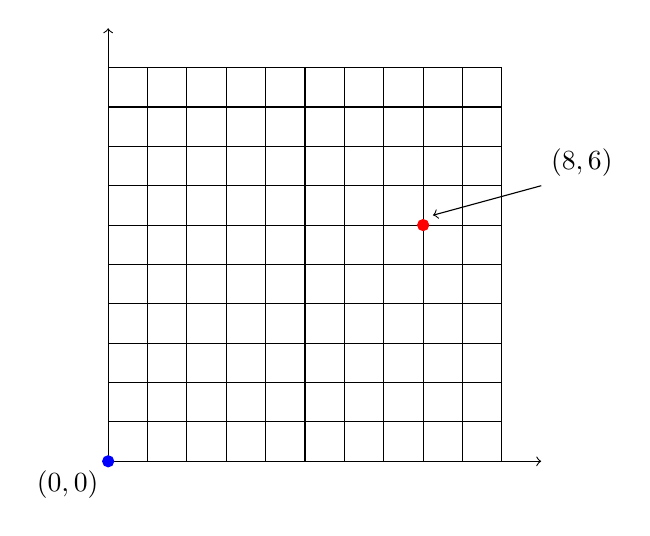
\begin{tikzpicture}[scale = 0.5]

        \draw [->] (0, 0) -- (0, 11);
        \draw [->] (0, 0) -- (11, 0);
        \draw (0, 0) grid (10, 10);

        \filldraw [color = blue] (0, 0) circle (4pt);
        \draw node [below left] {$(0, 0)$};

        \filldraw [color = red] (8, 6) circle (4pt);
        \draw [->] (11, 7) node [above right] {$(8, 6)$} -- (8.25, 6.25);

    \end{tikzpicture}
\end{center}

\begin{enumerate}[label = (\alph*)]

    \item Suppose each time the robot randomly moves right or up with equal chance.
    What is the probability that the robot will ever reach the point $(8, 6)$?

    \item Suppose another robot has a $\frac{2}{3}$ chance to move right and a $\frac{1}{3}$ chance to move up when $x + y$ is even, otherwise it has a $\frac{1}{4}$ chance to move right and a $\frac{3}{4}$ chance to move up.
    It stops whenever $|x - y| \geq 2$.
    Find the probability that $x - y = 2$ when it stops.

\end{enumerate}

\end{exercise}

% --------------------------------------------------------------------------------

\begin{solution}

\phantom{}

\begin{enumerate}[label = (\alph*)]
  \item The robot increases the sum $x + y$ by one in every step. That means, it can only
  reach the point $(8,6)$ in the fourteenth step and there are fourteen different places,
  where it can end up after fourteen steps.
  Therefore the probability can be calculated by a binomial distribution
  with $p = \frac{1}{2}$ and $n = 14$.
  \begin{align*}
    \P(\text{robot lands on} (8,6)) = \frac{1}{2^{14}}\binom{8}{14} = \frac{3003}{16384} \approx 0.1833.
  \end{align*}
  \item The robot can leave the corridor $|x - y| < 2$ only on every even turn.
  By induction, we show that the probability for leaving the corridor at $x - y = 2$,
  i.e. on the lower end of the corridor is $\frac{2}{5}$.

  \begin{align*}
    \P((2,0)) &= \frac{2}{3}\frac{1}{4} = \frac{2}{12} \\
    \P((1,1)) &= \frac{2}{3}\frac{3}{4} + \frac{1}{3}\frac{1}{4} = \frac{7}{12} \\
    \P((0,2)) &= \frac{1}{3}\frac{3}{4} = \frac{3}{12}.
  \end{align*}

  Therefore,
  \begin{align*}
    \P(\text{robot leaves corridor at lower end at second step}|
    \text{robot leaves corridor at second step})
    = \frac{2/12}{5/12} = \frac{2}{5}.
  \end{align*}

  After every even turn $2n$, supposing that the robot has not stopped, the only
  possible position remaining for the robot to be is $(n,n)$. \\

  The same calculation as beforehand show that the probability for leaving the corridor
  on the $2n + 2$nd step provided that the robot leaves the corridor is again $2/5$.
\end{enumerate}



\end{solution}

% --------------------------------------------------------------------------------
